\documentclass[
  a4paper,
  12pt,
  oneside,
  parskip=half,
  listof=totoc,
  bibliography=totoc,
  DIV=12,
  numbers=noenddot,
  BA.tex
  ]{subfiles}

\begin{document}

\section{Simulating the shift of reconstructed jets}

In section \ref{sec:hadron-triggers} it was mentioned that the behavior of jet clustering algorithms like the anti-$k_t$ algorithm depends on local quantities, like the underlying hadron density. The bigger the hadron density in a certain area in the $(\phi, \eta)$ phase space is the easier a clustered jet reaches a certain transverse momentum threshold because its $p_T$ consists of the transverse momenta of its constituents. Therefore jets tend to be clustered closer to the event plane where the soft hadron density is enhanced. It turns out the Pb--Pb event simulation, refer to section \ref{sec:event-simulation} for details, can be used to quantify how strongly the underlying soft background shifts the jet towards the event plane compared to where it would be clustered without any underlying background.

To accomplish this we first conduct jet clustering on a bare PYTHIA event that consists of jets but no soft hadron background to identify the leading jet. It has identified properties $(\phi_{\text{Leading}}, \eta_{\text{Leading}}, p_{T,\text{Leading}})$. Next the artificial soft hadron background is added to the PYTHIA event. The soft background is flow modulated and has a random event plane angle $\phi = \psi_m$. The leading jet has a distance of $d = \phi_{\text{Leading}} - \psi_m$ to the event plane. Now another jet clustering is performed on the event, giving new information on the leading jet $(\phi'_{\text{Leading}}, \eta'_{\text{Leading}}, p'_{T,\text{Leading}})$. The shift $\Delta \phi = \phi'_{\text{Leading}} - \phi_{\text{Leading}}$ is studied depending on the original distance of the leading jet to the event plane $d$. 

\subsection{Modeling the jet shift}
\label{sec:modeling-jet-shift}

\begin{figure}[H]
	\centering
	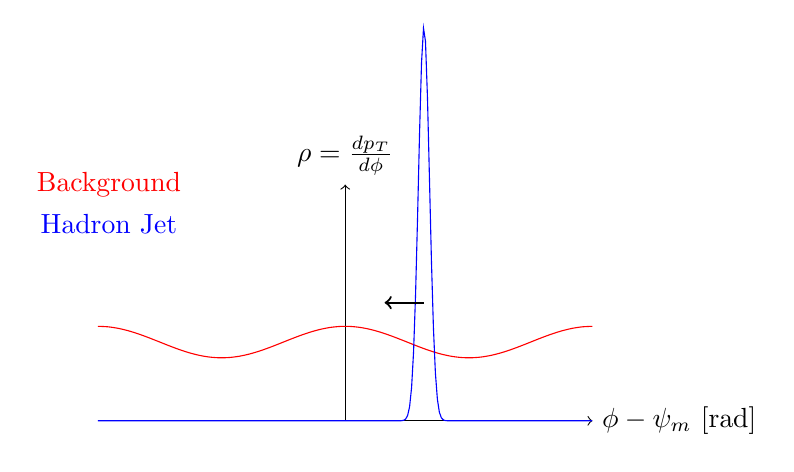
\begin{tikzpicture}
		%draw coordinate system
		\draw [->] (-3.14,0) -- (3.14,0)node[right] {$\phi - \psi_m$ [rad]};
		\draw [->] (0,0) -- (0,3) node[above] {$\rho = \frac{d p_T}{d \phi}$};
		%draw functions
		\draw [red] plot[domain=-3.14:3.14,
		samples = 50,
		smooth]({\x}, {1 + 0.2*cos((360/6.28)*2*\x)});
		\draw [blue] plot[domain=-3.14:3.14,
		samples = 250]({\x}, {5*exp(-((\x-1)*(\x-1))/0.01)});
		%draw labels
		\draw (-3,3) node[color=red] {Background};
		\draw (-3,2.5) node[color=blue] {Hadron Jet};
		%draw arrows
		\draw[->, thick](1,1.5)--(0.5,1.5);
		
	\end{tikzpicture}
	\caption{The transverse momentum densities of the background (subject to elliptic flow) and of the hadron jet in azimuthal direction. The jet is being produced independently from the underlying background. Because there are more soft hadrons to the left than to the right the jet clustered from PYTHIA+BG hadrons is more probably clustered farther left.}
	\label{fig:jetshiftmodel}
\end{figure}

To be able to judge the result of the analysis a simple model of the jet shift has to be introduced. Figure \ref{fig:jetshiftmodel} shows the overlay configuration of a jet and underlying soft hadron background that is subject to elliptic flow in the azimuthal direction. Due to symmetry reasons we do not expect the jet's azimuthal coordinate to change after adding background if either it is aligned with the event plane, so has $d=0$, or if it is aligned perpendicularly to the event plane. The most shift is expected if the soft hadron density asymmetry around the leading jet is greatest. 

Let us investigate the quantitative behavior closer. Because the jet radius $R$ is much smaller than the $v_2$ flow modulation spreads in azimuthal direction we can expand the underlying flow locally at the leading jet position according to

\begin{equation}
	\begin{gathered}
		\left. \rho_\text{BG}(\phi) \right|_{\phi_\text{Leading}} = \left. \frac{d p_T}{d (\phi - \psi_m)} \right|_{\phi_\text{Leading}} \propto \left. \frac{d N}{d (\phi - \psi_m)} \right|_{\phi_\text{Leading}} \\ \propto \left. 1 + 2 \sum_{n \geq 1}^{} v_n \cos(n (\phi - \psi_m)) \right|_{\phi_\text{Leading}}
		\stackrel{v_1 \ll v_2, v_n|_{n \geq 3} := 0}{\approx} \left. 1 + 2v_2 \cos(2(\phi - \psi_m)) \right|_{\phi_\text{Leading}}\\
		= \rho_0(\phi_\text{Leading}) + m \cdot (\phi - \phi_\text{Leading}) + \mathcal{O}(R^2) \text{ where } m \in \mathbb{R}
	\end{gathered}
	\label{eq:background_density}
\end{equation}

It is difficult to fully translate the anti-$k_t$ algorithm's behavior into an analytical model for many hadrons that are clustered. That is why we will look at how the algorithm clusters a jet in the few-particle limit where only one high-$p_T$ jet hadron is clustered with one low-$p_T$ hadron in the thermal background. The position of the low-$p_T$ hadron is determined based on where it appears most probably around the jet hadron according to equation (\ref{eq:background_density}). This is sufficient to prove the first-order linear behavior of the jet shift $\Delta \phi$ in $m$.

\paragraph{Local coordinate system}

Since the jet radius $R$ is small compared to the flow modulation and clustering only happens in a small azimuthal range it is appropriate to apply a small-angle approximation. For simplicity let us have the high-$p_T$ hadron, which we will call leading hadron for simplicity, to have $\phi_\text{Leading} := 0$ and the soft hadron to have the azimuthal coordinate $\phi_\text{h}$ (see figure \ref{fig:localcoord-shift}).

\begin{figure}[H]
	\centering
	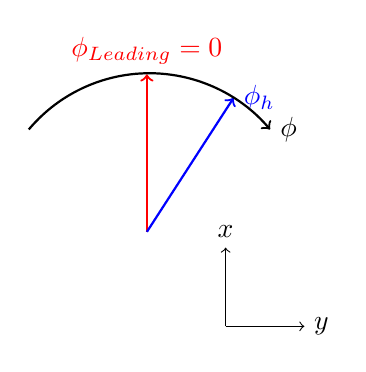
\begin{tikzpicture}
		
		% Particles
		\draw[thick , ->, red] (0,1) -- (0,3) node[above] {$\phi_\text{Leading} = 0$};
		\draw[thick , ->, blue] (0,1) -- (1.1,2.7) node[right] {$\phi_\text{h}$};
		
		% Winkelbogen oben
		\draw[thick, ->] (-1.5,2.3) arc[start angle=140,end angle=40,radius=2] node[right] {$\phi$};
		
		% Kleines Koordinatensystem unten rechts
		\begin{scope}[shift={(1,-0.2)}]
			\draw[->] (0,0) -- (0,1) node[above] {$x$};
			\draw[->] (0,0) -- (1,0) node[right] {$y$};
		\end{scope}
		
	\end{tikzpicture}
	\caption{The ALICE coordinate system with the high-$p_T$ jet at $\phi = 0$.}
	\label{fig:localcoord-shift}
\end{figure}

Following this definition the four-momenta of the leading hadron and the soft hadron are subsequently

\begin{equation}
	\begin{gathered}
		p_\text{Leading}^\mu = (E_\text{Leading}, p_{T,\text{Leading}}, 0, 0), \\
		p_\text{h}^\mu = (E_\text{h}, p_{T,\text{h}} \cos(\phi_\text{h}), p_{T,\text{h}} \sin(\phi_\text{h}), 0) \stackrel{R \ll \text{Flow modulation}}{\approx} (E_\text{h}, p_{T,\text{h}} (1-\frac{\phi_\text{h}^2}{2}), p_{T,\text{h}} \phi_\text{h}, 0)
	\end{gathered}
	\label{eq:four-momenta-approximation}
\end{equation}

\paragraph{Clustering}

The anti-$k_t$ algorithm will cluster the leading hadron with the soft hadron by adding up their four-momenta such that the four-momentum of the resulting clustered jet is

\begin{equation}
	\begin{gathered}
		{p'}^\mu_{\text{Leading}} = p_\text{Leading}^\mu + p_\text{h}^\mu \stackrel{(\ref{eq:four-momenta-approximation})}{\approx} (E_\text{Leading} + E_\text{h}, p_{T,\text{Leading}} + p_{T,\text{h}}(1 - \frac{\phi_\text{h}^2}{2}), p_{T,\text{h}} \phi_\text{h}, 0) .
	\end{gathered}
\end{equation}

The azimuthal coordinate of the clustered jet $\phi'_\text{Leading}$ can be calculated from the four-momentum ${p'}^\mu_{\text{Leading}}$ using the geometric relation between ($\phi, p_x, p_y$)

\begin{equation}
	\begin{gathered}
		\phi'_\text{Leading} \approx \tan(\phi'_\text{Leading}) = \frac{{p'}^2}{{p'}^1} = \frac{p_{T,\text{h}} \phi_\text{h}}{p_{T,\text{Leading}} + p_{T,\text{h}} (1-\frac{\phi_\text{h}^2}{2})} \stackrel{\phi_\text{h}^2 \ll R}{\approx} \frac{p_{T,\text{h}} \phi_\text{h}}{p_{T,\text{Leading}} + p_{T,\text{h}} } \propto \phi_\text{h}
	\end{gathered}
\end{equation}

\paragraph{The soft hadron's position}

The BG particle is generated based on $\rho_{BG}(\phi)$ in proximity to the jet within a jet radius $R$. The expected coordinate of the BG particle can be calculated according to

\begin{equation}
	\begin{gathered}
		<\phi_\text{h}> = \frac{\int_{-R}^{R} d\phi \, \phi \, \rho_{BG}(\phi)}{\int_{-R}^{R} d\phi \,  \rho_{BG}(\phi)} \stackrel{(\ref{eq:background_density})}{\propto} \int_{-R}^{R} d\phi \, \phi \, (\rho_0 + m \phi + \mathcal{O}(R^2)) = \frac{2}{3} m R^3 + \mathcal{O}(R^4) \propto m
	\end{gathered}
\end{equation}

\paragraph{Conclusion}

Thus, we can conclude that

\begin{equation}
	\begin{gathered}
		<\phi'_\text{Leading}> \propto <\phi_\text{h}> \propto m = \left. \frac{d \rho_{BG}(\phi)}{d \phi} \right|_{\phi_\text{Leading}} = - 4 v_2 \sin(2(\phi_\text{Leading} - \psi_m))
	\end{gathered}
\end{equation}

and we are left with the final formula for the jet shift with fit parameters $(A, \psi_m)$:

\begin{equation}
	\begin{gathered}
		<\Delta \phi> = <\phi'_\text{Leading} - \phi_\text{Leading}> = A \sin(2(\phi_\text{Leading} - \psi_m)) = A \sin(2 d)
	\end{gathered}
\end{equation}

\subsection{Jet shift in simulated Pb-Pb events}

\begin{figure}
	\centering
	\includegraphics[width=\linewidth]{Media/Plots/JetShiftResult.pdf}
	\caption{The shift of reconstructed jets towards the event plane in simulated Pb--Pb events.}
	\label{fig:jetshiftresult}
\end{figure}

Figure \ref{fig:jetshiftresult} shows the fitted results for the shift of reconstructed jets towards the event plane in simulated Pb--Pb events. The results are presented separately for different jet transverse momentum bins. The categorization was made before adding the soft hadron background. The general shape of the histogram resembles the expectations. Speaking in terms of figure \ref{fig:jetshiftmodel}: If the jet is right of the event plane it gets pulled to the left and vice versa. As expected soft jets are pulled less than hard jets because for harder jets an individual soft hadron contributes less to the total jet than for soft jets. The softest jets with $20.0 \leq p_{T,\text{Leading}} \leq 40.0 \bunit{GeV}$ are pulled by a maximum value of $d = 1.458 \cdot 10^{-2} \bunit{rad} = 0.836 \deg$. The jets are pulled hardest if they are approximately located where the local azimuthal elliptic flow changes the greatest, so for $d = \pm \pi/2$. The fit model that was derived in \ref{sec:modeling-jet-shift} approximately resembles the measured behavior, but does not fully explain the result. The shift tends to be greatest slightly off of $d = \pm \pi/2$. Reasons for this behavior could be truncation errors in the model derivation or that the linear behavior of the jet algorithm in the single particle approximation breaks down too quickly for more particles.

\end{document}